\chapter{Einleitung}


Durch den immer weiter fortschreitenden Umstieg auf erneuerbare Energien, werden gute Möglichkeiten zur Speicherung der gewonnenen Energie zunehmend wichtiger -- dies resultiert in einem entsprechend hohen Forschungsinteresse. Ein Vorschlag für eine neue Technologie ist die Nutzung von ionische Flüssigkeiten. Um aber am Ende effiziente Produkte herstellen zu können, müssen die physikalischen Vorgänge auf mikroskopischer Ebene verstanden sein. Dies betrifft insbesondere die Struktur und Dynamik von Molekülen und Atomen. 

Dafür kann die magnetische Kernspinresonanz (kurz NMR vom engl. „magnetic nuclear resonance“) eine hilfreiche Methode sein, ist sie doch beispielsweise für die Auflösung von Strukturen ein allgegenwärtig verwendetes Werkzeug von Chemikern. Aber auch die Möglichkeit, die Untersuchung auf ein bestimmtes Isotop zu beschränken, macht es möglich, den Einfluss der Dynamik von verschiedenen Komponenten eines Moleküls separat zu untersuchen.

In dieser Arbeit wurde Calciumrubidiumnitrat, kurz CRN, mit $^\text{87}$Rb-NMR untersucht. Dabei handelt es sich um ein Nitratsalz, welches bei entsprechend schnellem Abkühlen ein Glas, also einen amorphen Feststoff, bildet. Vorhergegangene Untersuchungen von CRN umfassen unter anderem die Untersuchungen von C. Zürn, welcher sich ebenfalls $^\text{87}$Rb-NMR beschäftigt hat \cite{zuern_paper} und auf dessen Ergebnisse diese Arbeit teilweise aufbaut.
\begin{figure}
	\begin{center}
		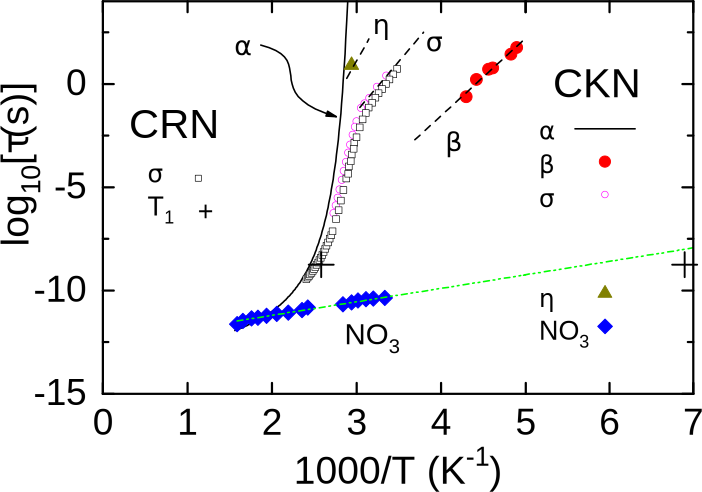
\includegraphics[width=.7\textwidth]{graphics/zuern/Plot1_b.pdf}
	\end{center}
	\caption{Relaxationskarte aus \cite{zuern_paper}, dargestellt in einem Arrhenius-Diagramm (logarithmierte Zeitkonstanten aufgetragen gegen die inverse Temperatur). Gezeigt sind ermittelte Zeitkonstanten aus Untersuchungen an CRN und CKN. Hierbei sind für diese Arbeit insbesondere der Betaprozess, dargestellt in rot, interessant. Die Daten hierzu stammen aus \cite{}} \label{fig:einl:zuernpaper}
\end{figure}

Eine Graph aus dem erwähnten Paper ist in Abbildung \ref{fig:einl:zuernpaper} zu sehen. Hier sind in CKN, kurz für Calciumkaliumnitrat, entdeckte Hinweise auf einen Betaprozess, dargestellt in rot, hervorzuheben. Die gestrichelte Linie durch die Punkte zeigt die lineare Fortsetzung der Punkte im Arrhenius-Diagramm an. Sollte dieser Trend standhalten, sollten bei Temperaturen in Bereichen kurz unter oder bei der Glasübergangstemperatur von $T_g = \SI{333}{K}$ Zeitkonstanten im hohen Mikrosekunden-Bereich zu erwarten sein. Zeitkonstanten dieser Größenordnungen lassen sich mit Methoden der NMR -- zum Beispiel der hier verwendeten Untersuchung von stimulierten Echos oder der Analyse von Linienformen von pulslängenabhängigen Spektren -- gut untersuchen.

Die Stoffe CKN und CRN ähneln sich sehr. Bis auf das gegen ein Rubidium-Atom ausgetauschte Kalium-Atom, welches der gleichen Hauptgruppe entstammt, teilen sie die gleiche Struktur, Glasübergangstemperatur und weitere Eigenschaften \cite{PIMENOV199793}. So ist beispielsweise auch in Abbildung \ref{fig:einl:zuernpaper} die Übereinstimmung von Leitfähigkeitsdaten $\sigma$ zwischen CRN und CKN zu erkennen. Daher ist es nachvollziehbar, für CRN und CKN ähnliche Zeitkonstanten eines Betaprozesses zu erwarten.

Während dieser Messungen wurde entdeckt, dass die Halbwertsbreite von CRN-Spektren zu höheren Temperaturen erst abnimmt -- was aufgrund der ansteigenden Bewegungsverschmälerung zu höheren Temperaturen zu erwarten ist -- aber bei Temperaturen ab $\SI{375}{K}$ wieder zunimmt. Dies widerspricht der naiven Erwartung, dass die Halbwertsbreite zu steigenden Temperaturen in diesem Fall lediglich abnehmen sollte. Um die Gründe dieses Phänomen zu klären wurden Spektren simuliert und ein Vergleich mit der Theorie der Quadrupol-Wechselwirkung zweiter Ordnung, welche hier entscheidende Einflüsse hat, durchgeführt.


Zunächst sollen in Kapitel \ref{chapter:theo} die theoretischen Grundlagen der NMR erläutert werden und eine Einführung in die Relaxation der Quadrupol-Wechselwirkung zweiter Ordnung gegeben werden. Kapitel \ref{chapter:simulation} beschreibt die für die Simulation verwendete Software mit zugehörigem Bewegungsmodell. Außerdem wird ein weiteres Bewegungsmodell vorgestellt, in der Zukunft facettiertere Untersuchungen ermöglichen könnte. In Kapitel \ref{chapter:exp_details} die verwendeten Apparaturen und Proben beschrieben, ehe in Kapitel \ref{chapter:experiment} die aufgenommenen Daten zunächst gezeigt, und dann ausgewertet und analysiert werden. Eine Zusammenfassung der Ergebnisse und ein Ausblick auf mögliche zukünftige Untersuchungen bilden den Abschluss der Arbeit.
